
\documentclass{article}
%************************************
\usepackage[utf8]{inputenc} 
\usepackage[total={18cm,24cm},centering]{geometry} 
\usepackage{natbib} 
\setcitestyle{super,open={},close={},citesep={,}} 

\usepackage[colorlinks,citecolor=blue,linkcolor=blue,urlcolor=blue]{hyperref} 
\usepackage{graphicx} 
\usepackage{tabularx} 
\usepackage{titlesec}
\titleformat*{\section}{\bf\centering\MakeUppercase}
\usepackage{authblk}

\newcommand\blankfootnote[1]{
  \begingroup
  \renewcommand\thefootnote{}\footnote{#1}
  \addtocounter{footnote}{-1}
  \endgroup
}

\title{\textbf{Estructuras de Datos y Base de Datos Relacionales}}

\author[1]{Brian Anco} 
\author[2]{Ericka Martínez}
\author[3]{José Contreras}

\affil[1]{Universidad Privada de Tacna, Perú. Email: briancoc@upt.pe}
\affil[2]{Universidad Privada de Tacna, Perú. Email: erimartinezy@upt.pe}
\affil[3]{Universidad Privada de Tacna, Perú. Email: joscontrerasm@upt.pe}

\date{}

%***************************************************************************************

\begin{document}
\maketitle

\begin{abstract}
    Las bases de datos son el método preferido para el almacenamiento estructurado de datos. Por Ello en este artículo se va Analizar de distintas bibliografías, tratando las estructuras de Datos, BD relacionales, Tipo de Estructuras de Datos, dentro de ello también se va tomar en cuenta: pila, árbol, lista enlazada, etc.\\Un sistema de gestión de bases de datos moderno es un sistema de software complejo que aprovecha muchos algoritmos sofisticados, por ejemplo, para evaluar operaciones relacionales, para proporcionar eficientes acceso a los datos. Viendo este tema extenso sobre la Estructura de Datos en base de Datos Relacionales, vamos definir su  amplia estructura y que tipos de datos tiene. 
\end{abstract}

\begin{abstract}
Databases are the preferred method for structured data storage. For this reason, this article will analyze different bibliographies, dealing with Data structures, relational DB, Type of Data Structures, within this it will also take into account: stack, tree, linked list, etc.\\A modern database management system is a complex software system that takes advantage of many sophisticated algorithms, for example, to evaluate relational operations, to provide efficient access to data. Seeing this extensive topic about the Data Structure in Relational Data, we are going to define its broad structure and what types of data it has.    
\end{abstract}


\section{Introducción}
Una base de datos relacional es una colección de elementos de datos organizados en un conjunto de tablas formalmente descritas desde la que se puede acceder a los datos o volver a montarlos de muchas maneras diferentes sin tener que reorganizar las tablas de la base.  

Una base de datos relacional consiste en un conjunto de tablas, a cada una de las cuales se le asigna un nombre exclusivo. Cada fila de la tabla representa una relación entre un conjunto de valores. Dado que cada tabla es un conjunto de dichas relaciones, hay una fuerte correspondencia entre el concepto de tabla y el concepto matemático de relación, del que toma su nombre el modelo de datos relacional. 
\newpage
\section{Desarrollo}
\subsection{Estructuras de Datos}
Se puede definir a la estructura de datos como una forma de representar la información de manera organizada. Estas no se limitan a únicamente mostrar la información, sino también poseen un comportamiento interno y cumplen con reglas específicas en cada estructura.
Buscar la eficiencia de los programas sigue siendo una de las características principales que deben tomar en cuenta los desarrolladores durante su elaboración, es por ello que el uso de las estructuras de datos en función a las necesidades del programa, representan una parte fundamental para alcanzar el objetivo de un programa eficiente.

\subsection{Bases de Datos Relacionales}
Una base de datos relacional nos permite almacenar y tener acceso a diferentes puntos de datos que están relacionados entre sí. Basada en el modelo relacional, cuenta con una manera directa e intuitiva de representar los datos en las tablas. Son altamente dinámicas, y la información se organiza en pequeñas partes integradas mediante identificadores, es por ello que tienen una mayor capacidad de almacenamiento, y son menos vulnerables a posibles fallas. 

\subsection{Tipos de Estructuras de Datos}
\subsubsection{Arrays}
Un array o arreglol (lista o tabla) es una secuencia de datos del mismo tipor Los datos se llaman elementos del array y se numeran consecutivamente 0, 1, 2, 3 . . . El tipo de elementos almacei nados en el array puede ser cualquier dato simple de Java o de un tipo previamente declarado como una clase. Normalmente, el array se utiliza para almacenar tipos tales como char, int: o float. (Zohonero Martínez, I. y Joyanes Aguilar, L. (2008). Estructuras de datos en Java. Madrid etc, Spain: McGraw-Hill España. Recuperado de https://elibro.net/es/ereader/bibliotecaupt/50117?page=87.)\\\\Los datos almacenados de un array son denominados elementos, y el número de elementos de un array son denominados tamaño o rango del vector. Para acceder a cada uno de los elementos de manera individual, se emplea un índice que definirá la posición del elemento dentro del vector, estos índices deben ser números enteros positivos. Gracias a ello, esta estructura nos permite acceder a sus elementos sin tener que consultar a elementos anteriores o posteriores, por lo que es más adecuada cuando se requiera acceder a los datos de manera aleatoria e impredecible. 
\begin{figure}[ht]
    \centering     
    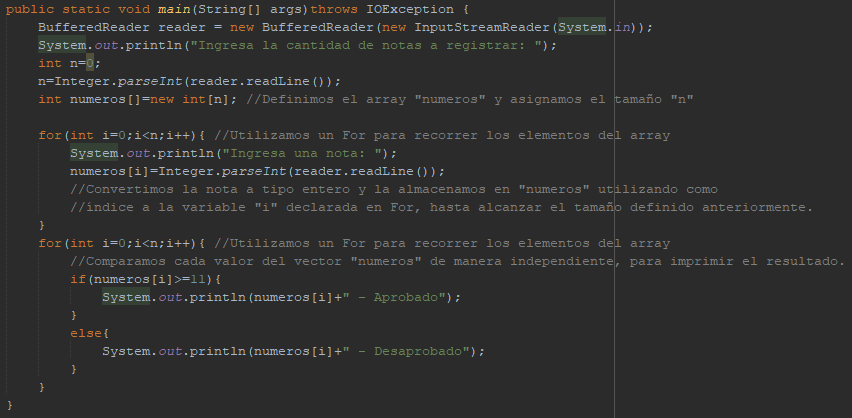
\includegraphics[height=8cm]{images/figura1.png}
    \caption{Declaración de un Array en Java.}
    \label{fig:BiasVoltage}
    
\end{figure}
\begin{figure}[ht]
    \centering     
    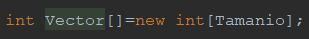
\includegraphics[height=0.5cm]{images/figura2.png}
    \caption{Declaración de un Array tipo entero en Java.}
    \label{fig:BiasVoltage}
    
\end{figure}

\subsubsection{Pilas}
Una pila es una estructura de datos de entradas ordenadas que sólo se pueden introducir y eliminar por un extremo, llamado cima. La pila se puede implementar guardando los elementos en un array, en cuyo caso su dimensión o longitud es fija. También se puede utilizar un Vector para almacenar los elementos. Otra forma de implementación consiste en construir una lista enlazada, de modo que cada elemento de la pila forma un nodo de la listar(Zohonero Martínez, I. y Joyanes Aguilar, L. (2008). Estructuras de datos en Java. Madrid etc, Spain: McGraw-Hill España. Recuperado de https://elibro.net/es/ereader/bibliotecaupt/50117?page=294.)

\begin{figure}[ht]
    \centering     
    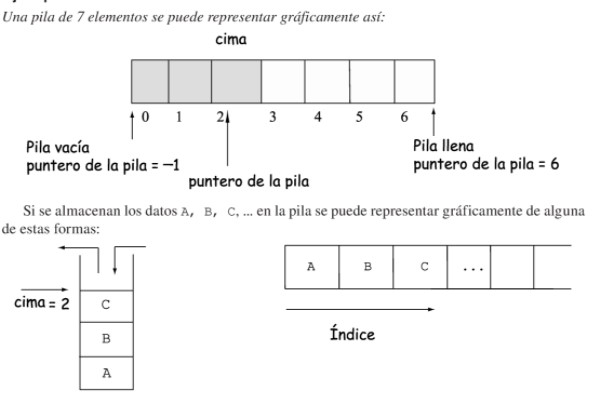
\includegraphics[height=5.5cm]{images/figura3.jpg}
    \caption{Estructura de una Pila.\\Fuente: Zohonero Martínez, I. y Joyanes Aguilar, L. (2008). Estructuras de datos en Java, pag 296.}
    \label{fig:BiasVqeoltage}
    
\end{figure}
\begin{figure}[ht]
    \centering     
    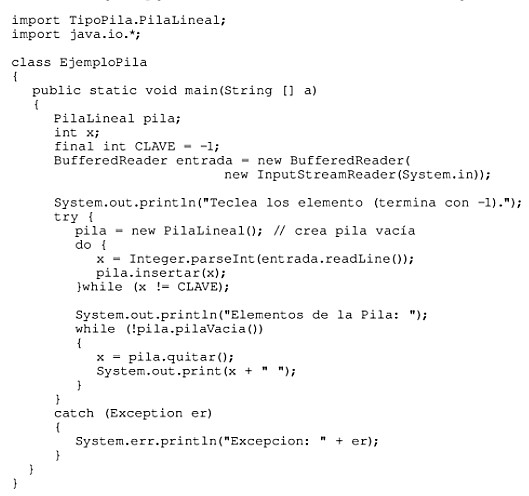
\includegraphics[height=8cm]{images/figura4.jpg}
    \caption{Desarrollo del ejemplo utilizando una Pila en Java.}
    \label{fig:BiasVoltager}
    
\end{figure}

\subsubsection{Colas}
Una cola es una estructura de datos cuyos elementos mantienen un cierto orden, de tal modo que sólo se pueden añadir elementos por un extremo, final de la cola, y eliminar o extraer por el otro extremo, llamado frente. (Zohonero Martínez, I. y Joyanes Aguilar, L. (2008). Estructuras de datos en Java. Madrid etc, Spain: McGraw-Hill España. Recuperado de https://elibro.net/es/ereader/bibliotecaupt/50117?page=319.)\\\\- La realización de una cola con un array lineal es notablemente ineficiente. se puede alcanzar la condición de cola llena existiendo elementos del array sin ocupar. Se aconseja no utilizar esta implementación.\\- Las bicolas son colas dobles, las operaciones básicas de insertar y retirar elementos se pueden realizar por los dos extremos, A veces se ponen restricciones de entrada o de salida realizar por algún extremo. Una bicola es realmente una extensión de una cola.
\begin{figure}[ht]
    \centering     
    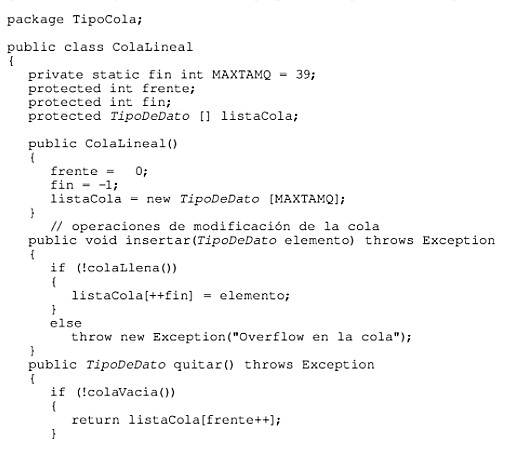
\includegraphics[height=8cm]{images/figura5.jpg}
    \caption{Declaración de la clase Cola - Parte 1}
    \label{fig:BiasVoltager}
    
\end{figure}
\begin{figure}[ht]
    \centering     
    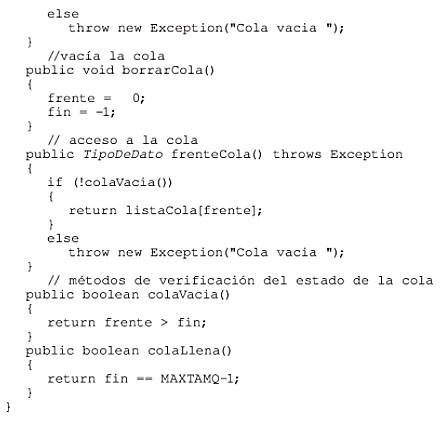
\includegraphics[height=8cm]{images/figura6.jpg}
    \caption{Declaración de la clase Cola - Parte 2}
    \label{fig:BiasVoltager}
    
\end{figure}


\subsubsection{Listas Enlazadas}
Una lista enlazada es una colección o secuencia de elementos dispuestos uno detras de otro, en la que cada elemento se conecta al siguiente elemento por un “enlace” o “referencia”, La idea básica consiste en construir una lista cuyos elementos, llamados nodos, se componen de dos partes (campos): la primera parte contiene la información y es, por consiguiente, un valor de un tipo generico (denominado Dato, TipoElemento, Info, etc), y la segunda parte es una referencia (denominado enlace o sgte) que apunta (enlaza) al siguiente elemento de la lista. (Zohonero Martínez, I. y Joyanes Aguilar, L. (2008). Estructuras de datos en Java. Madrid etc, Spain: McGraw-Hill España. Recuperado de https://elibro.net/es/ereader/bibliotecaupt/50117?page=251.)\\\\Las listas se pueden dividir en cuatro categorias:\\-Listas simplemente enlazadas. Cada nodo (elemento) contiene un único enlace que lo conecta al nodo siguiente o nodo sucesort La lista es eficiente en recorridos directos (“adelante”).\\- Listas doblemente enlazadas. Cada nodo contiene dos enlaces, uno a su nodo predecesor y otro a su nodo sucesort La lista es eficiente tanto en recorrido directo (“adelante”) como en recorrido inverso (“atras”).\\- Lista circular simplemente enlazada. Una lista enlazada simplemente en la que el último elemento (cola) se enlaza al primer elemento (cabeza) de tal modo que la lista puede ser recorrida de modo circular (“en anillo”).\\- Lista circular doblemente enlazada. Una lista doblemente enlazada en Ia que el último elemento se enlaza al primer elemento y viceversa. Esta lista se puede recorrer de modo circular (“en anillo”) tanto en dirección directa (“adelante”) como inversa (“atrás”).\\Ejemplo:

\begin{figure}[ht]
    \centering     
    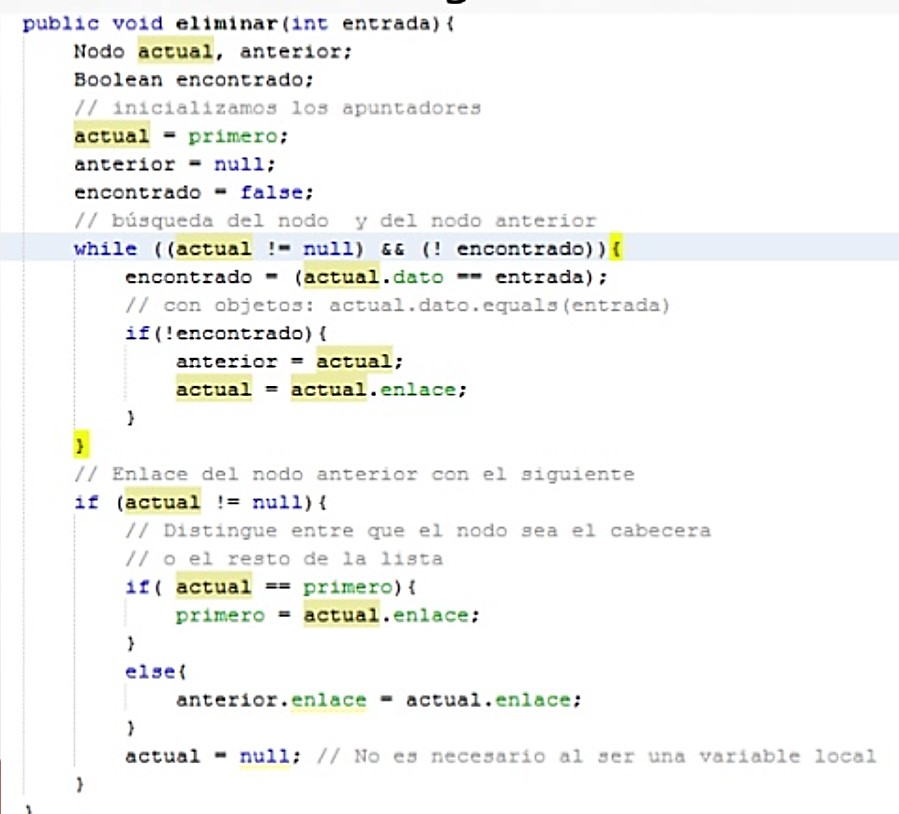
\includegraphics[height=10cm]{images/figura7.jpg}
    \caption{Ejemplo de Listas Enlazadas}
    \label{fig:BiasVoltager}
    
\end{figure}

\subsubsection{Árboles}
Un árbol consta de un conjunto finito de elementos, denominados nodos y de un conjunto finito de líneas dirigidas, denominadas ramas, que conectan los nodos. El número de ramas asociado con un nodo es el grado del nodo. (Zohonero Martínez, I. y Joyanes Aguilar, L. (2008). Estructuras de datos en Java. Madrid etc, Spain: McGraw-Hill España. Recuperado de https://elibro.net/es/ereader/bibliotecaupt/50117?page=393.)\\\\Un arbol es un conjunto de uno o más nodos, tales que:\\A) Hay un nodo diseñado especialmente llamado raiz.\\B) Los nodos restantes se dividen en n>=0 conjuntos distintos, T1 … Tn, tal que cada uno de estos conjuntos es un árbol. A T1 … Tn se les denomina subarboles del raiz.
\begin{figure}[ht]
    \centering     
    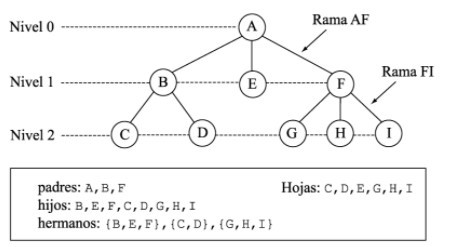
\includegraphics[height=6cm]{images/figura8.jpg}
    \caption{Terminología de árboles}
    \label{fig:BiasVoltager}
    
\end{figure}
Un árbol binario no puede tener más de dos subárboles. El recorrido de un árbol supone visitar cada nodo sólo una vez. En el recorrido preorden, el raíz se procesa antes que los subárboles izquierdo y derecho. Los árboles binarios ordenados, la búsqueda de una clave da lugar a un camino de búsqueda, de tal forma que baja por la rama izquierda si la clave buscada es menor que la clave de la raíz o baja por la rama derecha si la clave es mayor.
\begin{figure}[ht]
    \centering     
    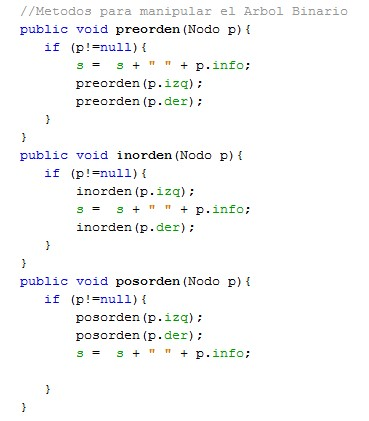
\includegraphics[height=10cm]{images/figura9.jpg}
    \caption{Ejemplo de Árboles}
    \label{fig:BiasVoltager}
    
\end{figure}


\subsubsection{Grafos}
Un grato permite modelar relaciones arbitrarias entre objetos. Un grato G = (V, A) es un par formado por un conjunto de vértices o nodos, V, y un conjunto de arcos o aristas, A. Cada arco es el par (u, w) , siendo u, w dos vértices relacionados. (Zohonero Martínez, I. y Joyanes Aguilar, L. (2008). Estructuras de datos en Java. Madrid etc, Spain: McGraw-Hill España. Recuperado de https://elibro.net/es/ereader/bibliotecaupt/50117?page=458.)\\\\La longitud de un camino es el número de arcos del camino. En un grato valorado, la longitud del camino con pesos es la suma de los pesos de los arcos en el camino.\\La matriz de adyacencia representa los arcos, relaciones entre un par de nodos de un grafo. Es una matriz de unos y ceros, que indican si dos vértices son adyacentes o no. Es una grado valorado, cada elemento representa el peso de la arista y por ello se la denomina matriz de pesos.
\begin{figure}[ht]
    \centering     
    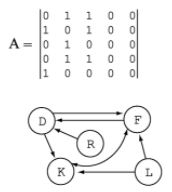
\includegraphics[height=4cm]{images/figura10.png}
    \caption{Grafo dirigido con los vértices\\Fuente: Zohonero Martínez,  I. y Joyanes Aguilar, L. (2008). Estructuras de datos en Java, pag 461.}
    \label{fig:BiasVoltager}
    
\end{figure}
\begin{figure}[ht]
    \centering     
    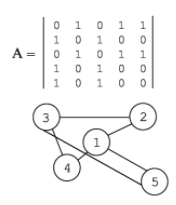
\includegraphics[height=4cm]{images/figura11.png}
    \caption{Grafo no dirigido con 5 vértices\\Fuente: Zohonero Martínez,  I. y Joyanes Aguilar, L. (2008). Estructuras de datos en Java, pag 461.}
    \label{fig:BiasVoltager}
    
\end{figure}
\begin{figure}[ht]
    \centering     
    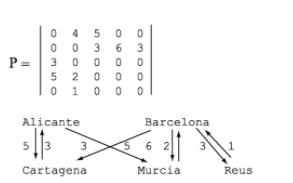
\includegraphics[height=4cm]{images/figura12.png}
    \caption{Grafo dirigido con factor de peso\\Fuente: Zohonero Martínez,  I. y Joyanes Aguilar, L. (2008). Estructuras de datos en Java, pag 461.}
    \label{fig:BiasVoltager}
    
\end{figure}
\section{Conclusiones}
Con este Articulo damos con concluido la estructura de Base de Datos Relacionales teniendo en cuenta las Bibliografías dadas de nuestra Asignatura, por ello analizando damos a conocer que existen varios tipos de estructuras de datos  para la BD, de acuerdo a qué tipo de BD deseamos realizar. Por ello aquí damos a entender en cómo se usa cada estructura y en cómo aplicar, a la vez colocamos conceptos concretos que dan a entender claramente nuestros objetivos.
\section{Recomendaciones}
Las Recomendaciones que podemos dar es tal que el tema ya que es muy extenso y con diversas bibliografías dadas, primero aplicamos en rescatar lo más importante de cada uno, luego hemos unido cada tema en el presente artículo, tuvimos temas complejos pero nada imposible.\\Fuera de ello, se recomienda tener una orden previa para poder hacer un artículo y siguiendo la plantilla real de Latex que pide. 
\bibliographystyle{ieeetr}
\bibliography{references}

\end{document}
